\documentclass[a4paper]{article}

%% Language and font encodings
\usepackage[T1]{fontenc}
\usepackage[utf8x]{inputenc}
\usepackage[english]{babel}

\usepackage[colorlinks=true, allcolors=blue]{hyperref}

\urlstyle{tt}
\newcommand{\email}[1]{\href{mailto:#1}{\tt{\nolinkurl{#1}}}}
\newcommand{\orcid}[1]{ORCID: \href{https://orcid.org/#1}{\tt{\nolinkurl{#1}}}}

\newcommand{\figleg}[1]{\centering\itshape{#1}\/}
\newcommand{\figref}[1]{(see figure~\ref{#1})}

\usepackage[sfdefault,lf]{carlito}
%% The 'lf' option for lining figuressy
%% The 'sfdefault' option to make the base font sans serif
\usepackage[parfill]{parskip}
\renewcommand*\oldstylenums[1]{\carlitoOsF#1}%
\usepackage{fancyhdr}
\usepackage{natbib}
\usepackage{authblk}
\setlength{\headheight}{41pt}

%% Sets page size and margins
\usepackage[a4paper,top=3cm,bottom=2cm,left=3cm,right=3cm,marginparwidth=1.75cm]{geometry}

%% Useful packages
\usepackage{amsmath}
\usepackage{graphicx}
\usepackage{booktabs}
\usepackage{caption}
\usepackage{subcaption}

\usepackage[colorinlistoftodos]{todonotes}

\fancyhead[L]{Posted: \today}
\fancyhead[R]{

\includegraphics[width=4cm]{img/engrXiv_banner.png}
}
\pagestyle{plain}
\title{Adaptive Removal of the Transcranial Alternating Current Stimulation Artifact from the Electroencephalogram}
\author[1,*]{Robert Guggenberger}
\author[1]{N.N.}
\affil[1]{Department for Translational Neurosurgery, University Hospital Tübingen}

\affil[*]{Corresponding author: \email{robert.guggenberger@posteo.eu}}
\date{\today}

\usepackage{varioref}
\usepackage{hyperref}
\usepackage{cleveref}
\hypersetup{hidelinks = true}

\usepackage[nonumberlist,acronym]{glossaries}
% abbreviations:
\newacronym{eeg}{EEG}{electroencephalogram}
\newacronym{tacs}{tACS}{transcranial alternating current stimulation}
\newacronym{tms}{TMS}{transcranial magnetic stimulation}
\newacronym{tpca}{tPCA}{temporal principal component analysis}
\newacronym{sma}{SMA}{superposition of moving averages}
\makeglossaries{}

% --------------------------------------------------------------------------
\begin{document}
\maketitle
\thispagestyle{fancy}

\begin{abstract}
Your abstract.
\end{abstract}

\section{Introduction}

The combination of \gls{tacs} and \gls{eeg} has been explored in several recent studies. While the analysis of \gls{eeg} before or after stimulation posits limited technical challenges, the \gls{eeg} recording during stimulation is heavily affected by the stimulation artifact.

\subsection{Matched Phase and Frequency}
Computational simulations suggest that the power of endogenous oscillations would increase most if the frequency of~\gls{tacs} matches the targets eigenfrequency~\citep{Kutchko_2013,Zaehle_2010}.
This has been supported by evidence from animal studies~\citep{Schmidt_2014}, and human studies combining \gls{tacs} with \gls{tms} \citep{Guerra_2016}, or contrasting pre and post resting state power analysis \citep{Zaehle_2010}.
It has also been suggested that the phase of neuronal populations would be locked to the phase of the \gls{tacs} signal \citep{Reato_2013}. This has been supported by evidence from studies combining \gls{tacs} with motor output \citep{Brittain_2013}, \gls{tms}~\citep{Raco_2016,Nakazono_2016} or sensory perception~\citep{Gundlach_2016}.

This suggests that the effect of \gls{tacs} can result in neurophysiological effects which are phase-and frequency-matched to the stimulation artifact. Such frequency and phase matching between \gls{tacs} and \gls{eeg} recordings can render the removal of the artifact difficult or impossible, as the signal might no longer be separatable from the artifact.

\subsection{Non-Stationary Amplitude Modulation}

An approach to tackle this issue is to assess the time-course of the~\gls{eeg} signal. Consider the assumption that the artifact is stationary and superpositioned on the physiological signal. Then, modulations in the amplitude of the recorded~\gls{eeg}-signal must be caused by changes in the underlying physiology.
This would be the case, even if frequency and phase are matched to the stimulation signal. Approaches assuming such stationarity of the stimulation artifact have been used e.g.\ by~\cite{Pogosyan_2009}.

Yet, detailed analysis of the stimulation artifact provides evidence that the artifact amplitude is actually not stationary. Instead, the amplitude is modulated by heart-beat and respiration~\citep{Noury_2016}. It has been argued that unregularized spatial filters might be able to remove this amplitude modulation~\citep{Neuling_2017}. But if only few channels are recorded, the method can fail, as the estimation of the spatial covariance is insufficient, or impossible in the single-channel-case.
Consider furthermore that event-related responses like modulation of skin impedance can also affect the scalp conductance at stimulation electrodes. This would introduce event-related amplitude modulation of the stimulation artifact. In that regard, disentangling true signal from the stimulation artifact stays technically challenging.

\subsection{Artifact Distortion}

Ideally, the stimulation artifict of~\gls{tacs} resembles a sinusoid. Yet, practical experience suggests that the signal is usually distorted to various degrees.
Figure~\ref{fig:nonsinus} shows examples of distortion and saturation in two recordings of \gls{tacs}-\gls{eeg}. The gray traces indicate nine invididual periods, while the red trace indicates their average. In figure~\ref{fig:distortion}, note the periodic, yet non-sinusoidal waveform. In figure~\ref{fig:saturation}, note the saturation.

\begin{figure}[hbtp]
    \begin{subfigure}{.5\textwidth}
    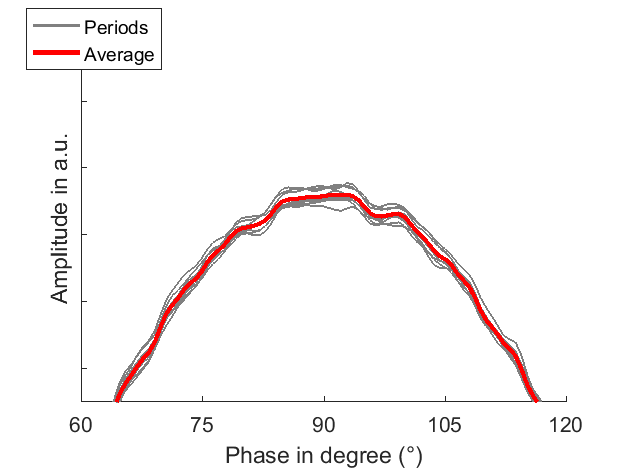
\includegraphics[width=\textwidth]{./img/intro/distortion.png}
    \caption{Distortion}\label{fig:distortion}
    \end{subfigure}
    \begin{subfigure}{.5\textwidth}
    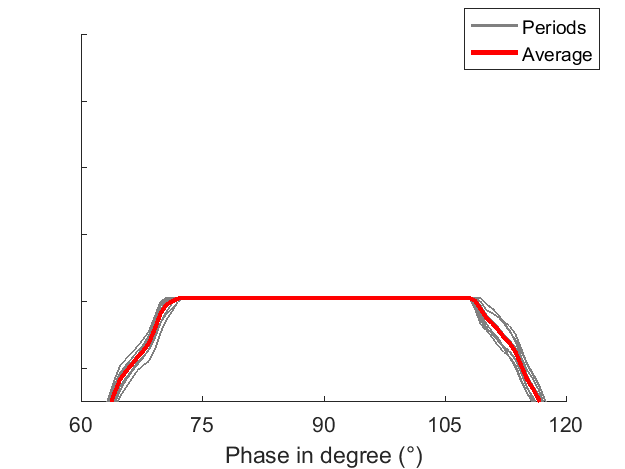
\includegraphics[width=\textwidth]{./img/intro/saturation.png}
    \caption{Saturation}\label{fig:saturation}
    \end{subfigure}
    \caption{Examples for loss of sinusoidal fidelity}\label{fig:nonsinus}
\end{figure}

The temporally and spatially uneven impedance distribution has been suggested as cause of distortion, rendering the resulting waveform periodic, but non-sinusoidal. A major problem is amplifier saturation, i.e.\ the stimulation artifact exhibiting an amplitude to large for the dynamic range of the amplifier, causing the signal to be cut off and information to be lost.
Additionally, non-linearites in the amplifier slew rate can distort the shape even when the signal is close to the saturation threshold. Recently, non-linearities in how stimulators control the applied current has been suggest as further source of modulation~\citep{Neuling_2017}.

\subsection{Computational Demands}

Methods based on adaptive template construction and \gls{tpca}~\citep{Niazy_2005} have been explored for removal of  non-stationary and misshaped \gls{tacs} artifacts~\citep{Helfrich_2014}.  Consider that the process of template construction, the estimation of accurate weights for removal by template subtraction and the suqsequent removal of residual artifacts using \gls{tpca} is computationally cumbersome. Additionally, it often requires off-line analysis supported by visual inspection.
Such a multi-staged template-approach is therefore of limited utility for on-line artifact removal. Furthermore, critical evaluation has suggested that the residual artifact spans several principal components, and a sufficient artifact removal is therefore not possible with \gls{tpca} \citep{Noury_2016}.

\subsection{Rationale}

We were interested in development of a computationally fast approach, feasible for online artifact removal. At the same time, the approach was required to account for the dynamical modulation of the artifact amplitude, and the possibility of non-sinusoidal distortion and saturation. Ideally, the approach should allow to estimate physiological signals at the frequency of stimulation, even if physiological oscillations were phase-locked to the stimulation signal.

\section{Approach}

The main idea is that at any given time point $t$, the recorded signal $r(t)$ is a linear super\-position of a neurophysiological signal $n(t)$, the stimulation artifact $a(t)$ and a white noise term $e(t)$. The task is to recover $n(t)$ by estimating $a(t)$ and $e(t)$ and subtracting from $r(t)$.

\begin{eqnarray}
    r(t) = n(t) + a(t) + e(t)\\
    n(t) = r(t) - a(t) - e(t)
\end{eqnarray}

\subsection{Periodic Estimation}
Assume that the~\gls{tacs} artifact were \emph{non-sinusoidal}, but \emph{stationary and periodic}. At the same time, assume that neurophysiological signals $n$ were absent. Then, we could estimate the amplitude of $a$ at any time-point $t$ by using the recorded signal $r$ any~\gls{tacs} one period length $p$ earlier~\eqref{eq:Comb}.
Subtraction of a delayed version of the signal is also known as comb filter. Please note that for discretely sampled signals, this approach only works if the frequency of the artifact is an integer divisible of the sampling frequency.

\begin{equation}
    \hat{a}(t) = r(t-p)\label{eq:Comb}
\end{equation}

\subsubsection{Uniform Comb Filter}

Consider that white noise term $e$ is still superpositioned on $r$.  Because white noise $\langle e\rangle$ converges asymptotically to zero with increased sample size, an approach to estimate the artifact amplitude could be to average across as many earlier periods as possible~\eqref{eq:Average}. Subsequently, this estimate can be used to  remove the artifact from $r$.
In real applications, stimulation duration is limited and computational constraints exist. This is reflected by the fact that we have to use a finite number for $N$.

\begin{equation}
    \hat{a}(t) = \sum_{n=1}^{N} \frac{r(t - np)}{N}\label{eq:Average}
\end{equation}

\subsubsection{Superposition of Moving Averages}

Please note that averaging across neighbouring periods $M$~\eqref{eq:SMA} has been suggested before and termed~\gls{sma} by~\cite{Kohli_2015}.

\begin{equation}
    \hat{a}(t) = \sum_{n-M/2}^{n+M/2} \frac{r(t - np)}{M+1}\label{eq:SMA}
\end{equation}

Consider that the approach using only past values~\eqref{eq:Average} returns a causal filter. Applied online, a causal filter would be able to remove the artifact without the delay of $(Mp)/2$ necessary for~\gls{sma}. Furthermore,~\gls{sma} is well-defined only for even $M$. This motivates the exploration of causal filters for artifact removal.

\subsection{Decay Weighting}

More importantly, the artifact amplitude has been described to be non-stationary  and dynamically modulated~\citep{Noury_2016,Neuling_2017}.
For real applications, equation~\eqref{eq:Average} can therefore return a biased estimate, depending on whether the integral of this modulation over the time-period $N\times p$ converges to zero.
One attempt to tackle with this issue can be the use of a time-dependent weighting function instead of a constant $N$~\eqref{eq:Weighted}, with the weighting function designed to reduce a possible bias.

\begin{equation}
    \hat{a}(t) = \sum_{n=1}^{N} w_n r(t - np)\label{eq:Weighted}
\end{equation}

If the dynamics behind the modulation of the artifacts amplitude are known or can be estimated sufficiently, an optimal weighting function can be constructed. Although it has been suggested that there are event-dependent component of the amplitude modulation (e.g.\ by heartbeat or respiration~\cite{Noury_2016} or stimulator impedance check~\cite{Neuling_2017}), the dynamical system governing the event-independent amplitude modulation are usually unknown.

Consider for example a simple comb filter, where we remove the artifact by subtracting the value sampled from any earlier period. Assume now that this values is drawn uniform at random from the last $N$ periods.\footnote{Note, that in the case of full stationarity for the last $N$ periods, its expected performance in the long is expected to be similar to averaging}
If the system is fully stationary for the last $N$ periods, performance is virtually identical to the comb filter based on averaging~\eqref{eq:Average}. If it is governed by a stochastic process (at least for the last time-points $N$), e.g.\ a Wiener process, the precision of the estimate degrades as a function of the delay. This rationale justifies non-uniform weights.
In the case of the uniform sampling, we have a single shape parameter $N$, defining how far back we trust a measurement to have the same precision as earlier samples. By controlling the parameters of alternative weight functions, we might better match the stochastic process governing the amplitude modulation. This might allows us to achieve a better artifact estimation and subsequent removal.

The qualifying criteria for these weighting functions are that the sum of all their weights should be equal to one. This keeps the weighting function in agreement with the average~\eqref{eq:Average}, returns an unbiased estimate in the case of full stationarity, and keeps the filter stable. In the following sections, we will discuss three weighting functions assuming non-skewed and unbiased generating processes.

\subsubsection{Linear Weighting}

One approach is linearization, e.g.\ using a linear decreasing weighting function.  The necessary normalization can easily be implemented by using the triangular number for a given $N$ as normalizing constant $k$~\eqref{eq:NormLinear}. Hence, equation~\eqref{eq:Linear} returns weights for earlier periods based on a linear temporal weight decay.

\begin{equation}
    w_n = \frac{N-n+1}{k}\label{eq:Linear}
\end{equation}
with the following normalization
\begin{equation}
    k  = \sum_{n=1}^{n} n = \frac{N(N+1)}{2}\label{eq:NormLinear}
\end{equation}

\subsubsection{Exponential Weighting}

Motivated by the fact that exponentials are an essential building block of signal processing and especially powerful for decay anaylsis, an alternative approach could be an exponential weighting function. The time constant $\tau$ of an exponential controls its decay across time. To maintain the shape across different $N$, we consider it reasonable to normalize $n$ by $N$. Hence, equation~\eqref{eq:Exp} returns weights for earlier periods based on their exponential temporal weight decay.

\begin{equation}
    w_n = \frac{1}{k} e^{\tau-\tau{(n/N)}}\label{eq:Exp}
\end{equation}
with the following normalization
\begin{equation}
    k  = \sum_{n=1}^{N} e^{\tau-\tau{(n/N)}}\label{eq:NormExp}
\end{equation}

\subsubsection{Gaussian Weighting}

Assuming the the precision of the estimate decreaeses over time, a sampling-distribution rationale motivates a Gaussian weighting function. Using a suitable parameterization, and centering on zero, the inverse of the standard deviation $\frac{1}{\sigma^2}$ defines the time constant $\tau$ of a Gaussian distribution, which controls its decay.
To maintain the shape across different $N$, we consider it again reasonable to normalize $n$ by $N$. Hence, equation~\eqref{eq:Gauss} returns weights for earlier periods based on their exponential temporal weight decay.

\begin{equation}
    w_n = \frac{1}{k} f(n/N)\label{eq:Gauss}
\end{equation}
with the following generating function and normalization
\begin{align}
    f(x)  & = \sqrt{\frac{\tau}{2\pi}} e^{-(\tau x^2)/2}  \\
    k  & = \sum_{n=1}^{N} f(n/N)\label{eq:NormGauss}
\end{align}

\subsection{Examples}

We implemented functions for kernel creation and artifact removal in Matlab 2016b. Additionally, we evaluated them  on simulated and real data. Code\footnote{\url{https://github.com/agricolab/ARtACS}} and data has been published online.

\subsubsection{Exemplary Causal Kernels}

Examine the following exemplary kernels constructed for a sampling rate of 1KHz, a stimulation frequency of 10 Hz and a memory of 10~\ref{fig:ExemplaryCausalKernels}.

\begin{figure}[hbtp]
    \begin{subfigure}{.245\textwidth}
        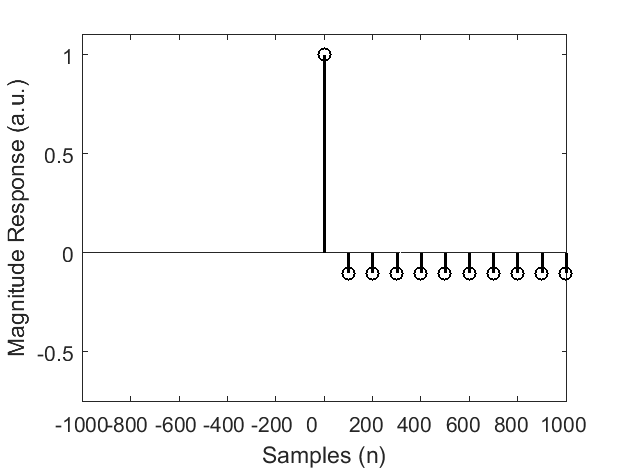
\includegraphics[width=\textwidth]{img/causal/kernel_ave.png}\\
        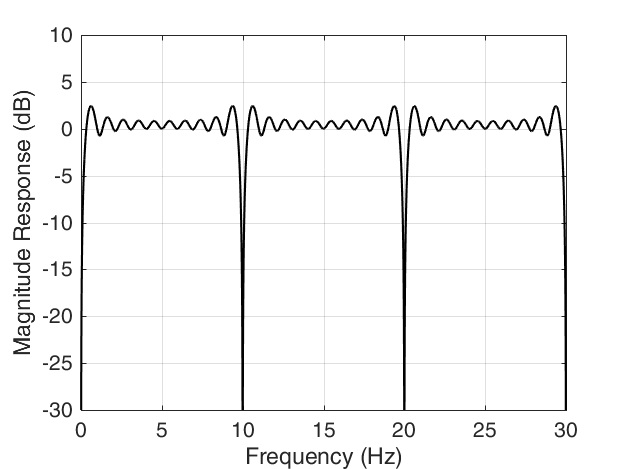
\includegraphics[width=\textwidth]{img/causal/mag_ave.png}
        \caption{Uniform}\label{fig:UniformKernel}
    \end{subfigure}
    \begin{subfigure}{.245\textwidth}
        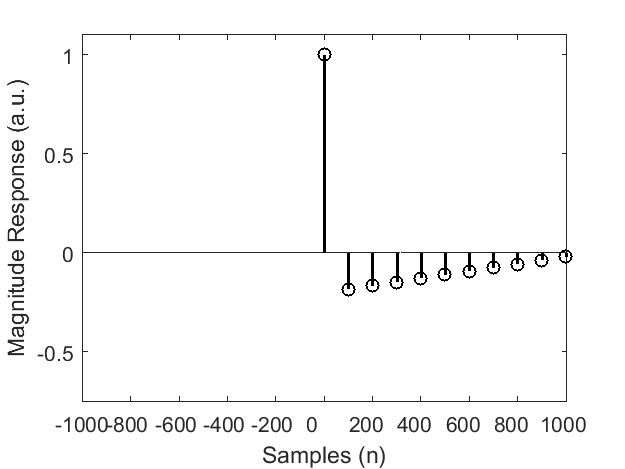
\includegraphics[width=\textwidth]{img/causal/kernel_linear.png}\\
        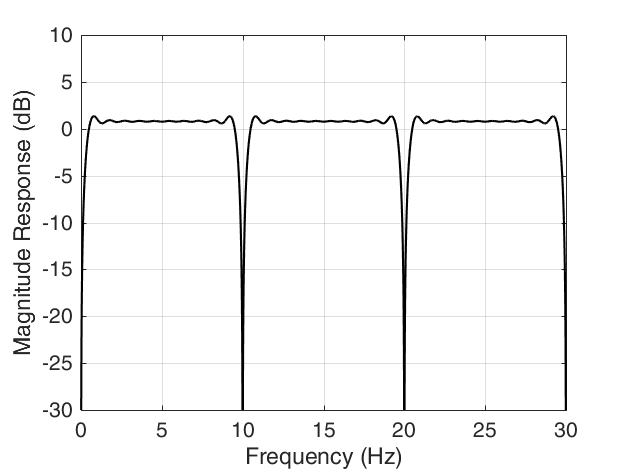
\includegraphics[width=\textwidth]{img/causal/mag_linear.png}
        \caption{Linear}\label{fig:LinearKernel}
    \end{subfigure}
    \begin{subfigure}{.245\textwidth}
        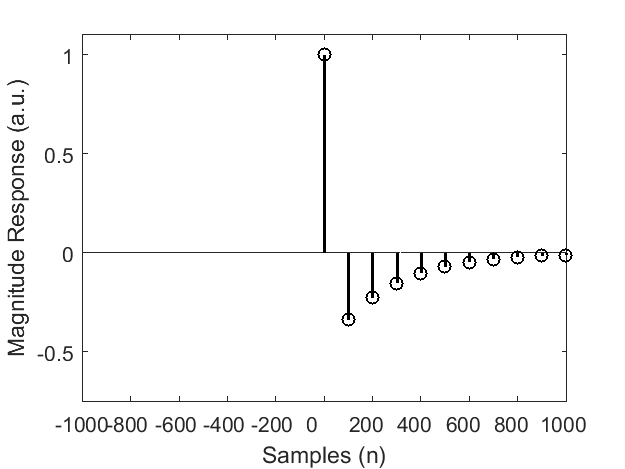
\includegraphics[width=\textwidth]{img/causal/kernel_exp.png}\\
        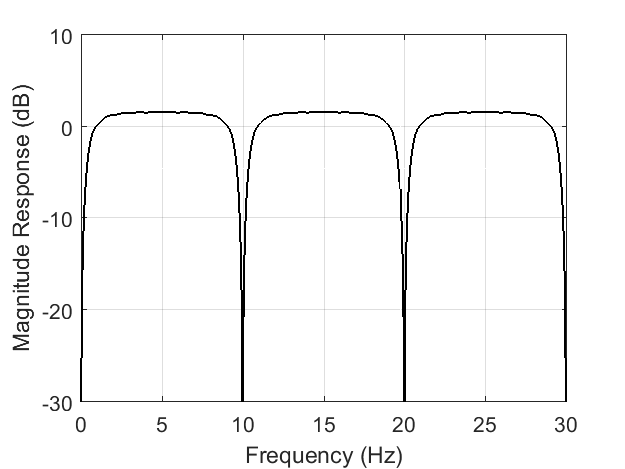
\includegraphics[width=\textwidth]{img/causal/mag_exp.png}
        \caption{Exponential~$\tau=4$}\label{fig:ExponentialKernel}
    \end{subfigure}
    \begin{subfigure}{.245\textwidth}
        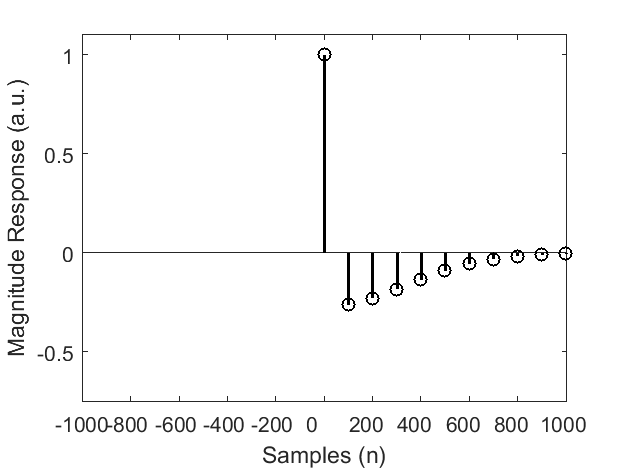
\includegraphics[width=\textwidth]{img/causal/kernel_gauss.png}\\
        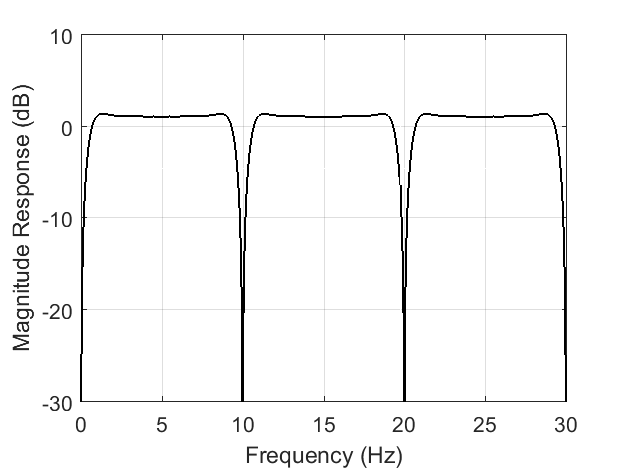
\includegraphics[width=\textwidth]{img/causal/mag_gauss.png}
        \caption{Gaussian~$\tau=3$}\label{fig:GaussKernel}
    \end{subfigure}
    \caption{Exemplary Causal Kernels}\label{fig:ExemplaryCausalKernels}
\end{figure}

As you can see from figure~\ref{fig:ExemplaryCausalKernels}, the (numerically calculated) magnitude responses of the four approaches are highly similar. Their key characteristic is the strong supression of the target frequency and its integer multiples.
Yet, note the difference in passbands. We find strong ringing in the passband for the uniform~\ref{fig:UniformKernel} and linear kernel~\ref{fig:LinearKernel}, especially compared to the smooth transitions of the exponential~\ref{fig:ExponentialKernel} or Gaussian kernels~\ref{fig:GaussKernel}.


\subsubsection{Exemplary Symmetric Kernels}

Examine the following exemplary kernels constructed with parameters identical to the causal kernels, but symmetric on the origin instead~\ref{fig:ExemplarySymKernels}. Please note that a uniform symmetric would be a~\gls{sma}-Kernel~\eqref{eq:SMA}.

\begin{figure}[hbtp]
    \begin{subfigure}{.245\textwidth}
        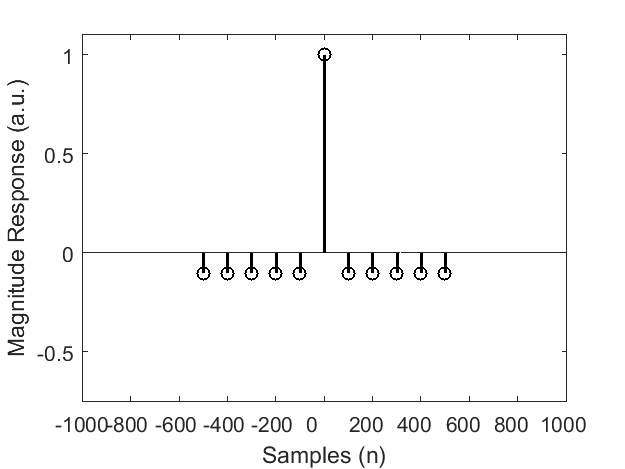
\includegraphics[width=\textwidth]{img/sym/kernel_ave.png}\\
        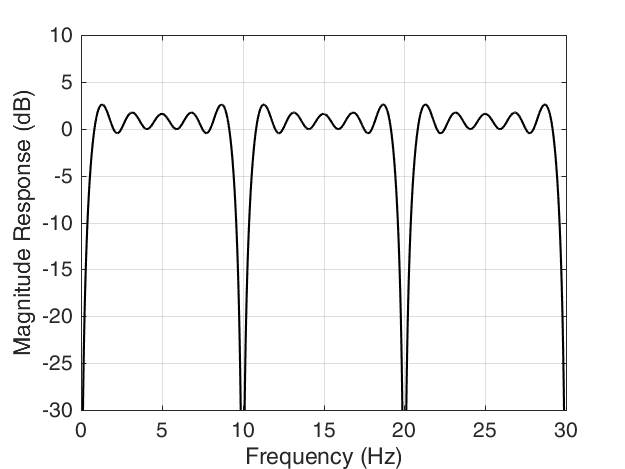
\includegraphics[width=\textwidth]{img/sym/mag_ave.png}
        \caption{Uniform}\label{fig:UniformSymKernel}
    \end{subfigure}
    \begin{subfigure}{.245\textwidth}
        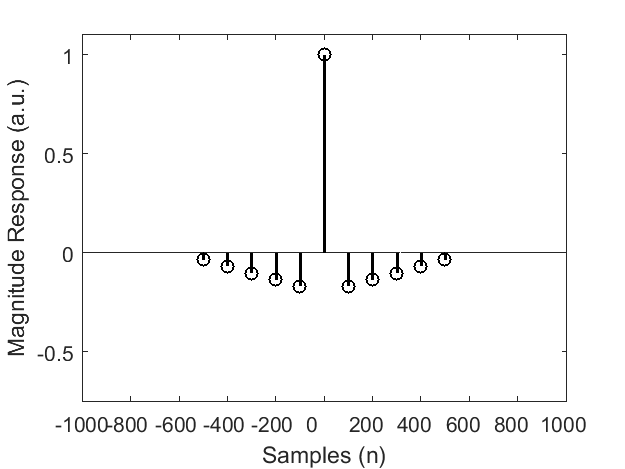
\includegraphics[width=\textwidth]{img/sym/kernel_linear.png}\\
        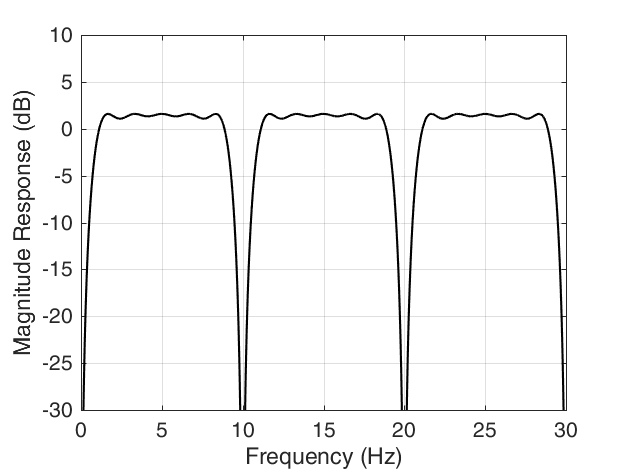
\includegraphics[width=\textwidth]{img/sym/mag_linear.png}
        \caption{Linear}\label{fig:LinearSymKernel}
    \end{subfigure}
    \begin{subfigure}{.245\textwidth}
        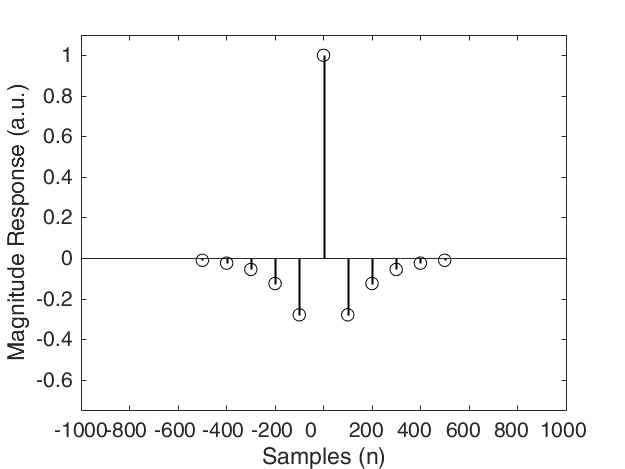
\includegraphics[width=\textwidth]{img/sym/kernel_exp.png}\\
        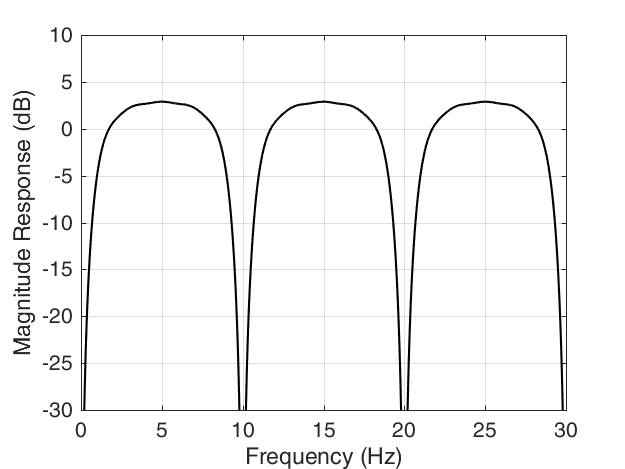
\includegraphics[width=\textwidth]{img/sym/mag_exp.png}
        \caption{Exponential~$\tau=4$}\label{fig:ExponentialSymKernel}
    \end{subfigure}
    \begin{subfigure}{.245\textwidth}
        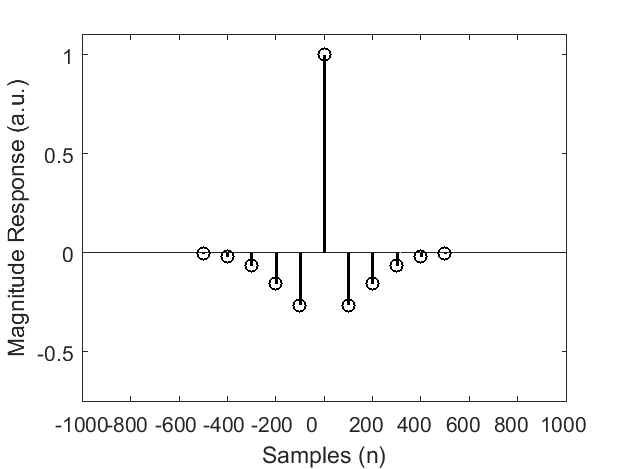
\includegraphics[width=\textwidth]{img/sym/kernel_gauss.png}\\
        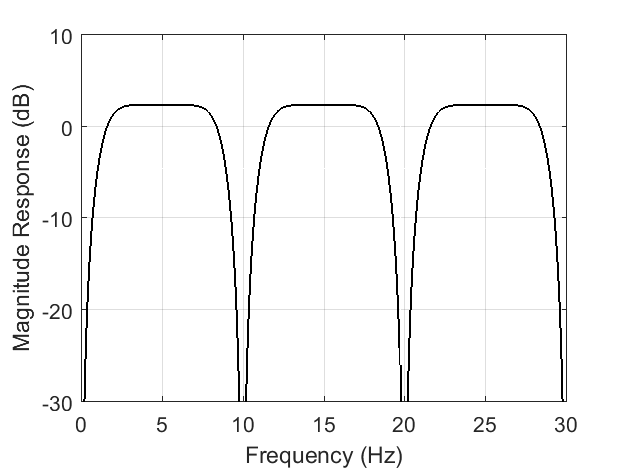
\includegraphics[width=\textwidth]{img/sym/mag_gauss.png}
        \caption{Gaussian~$\tau=3$}\label{fig:GaussSymKernel}
    \end{subfigure}
    \caption{Exemplary Symmetric Kernels}\label{fig:ExemplarySymKernels}
\end{figure}

As you can see from figure~\ref{fig:ExemplarySymKernels}, symmetric kernels share key characteristic with the causal kernels, especially the strong suppression. But we also find the presence of ringing for the the uniform~\ref{fig:UniformSymKernel} and linear kernel~\ref{fig:LinearSymKernel}. Note that the passband range appears to be  less narrow for the symmetric compared to the causal filters. Yet the passband response for the Gaussian Kernel exhibits  superior flatness~\ref{fig:GaussSymKernel}.


\subsubsection{Exemplary Kernel Tuning}

Examine the following exponential kernels constructed with different $\tau$~\figref{fig:ExemplaryTauTuning} and $N$~\figref{fig:ExemplaryNPTuning}.

\begin{figure}[hbtp]
    \begin{subfigure}{.33\textwidth}
        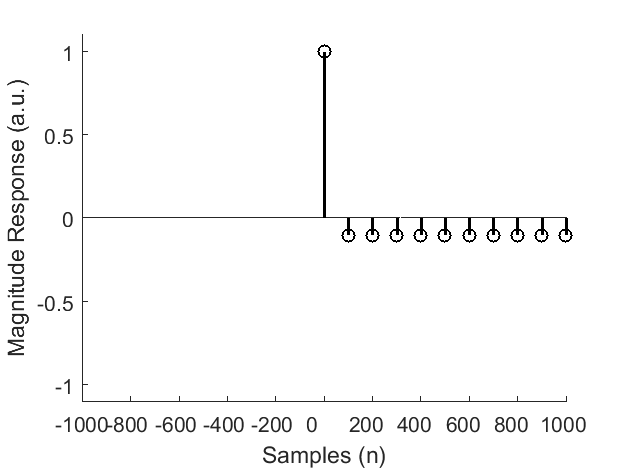
\includegraphics[width=\textwidth]{img/tau/kernel_exp_0.png}\\
        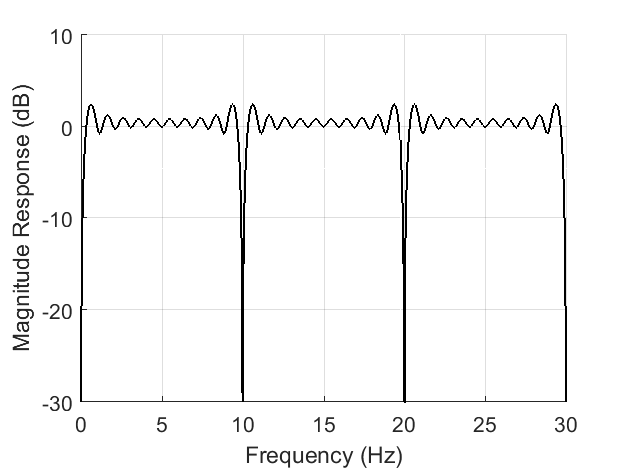
\includegraphics[width=\textwidth]{img/tau/mag_exp_0.png}
        \caption{Exponential~$\tau=0$}\label{fig:ExpTau0}
    \end{subfigure}
    \begin{subfigure}{.33\textwidth}
        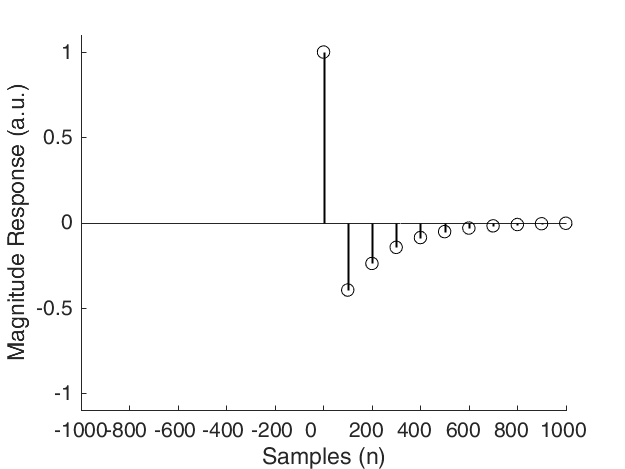
\includegraphics[width=\textwidth]{img/tau/kernel_exp_5.png}\\
        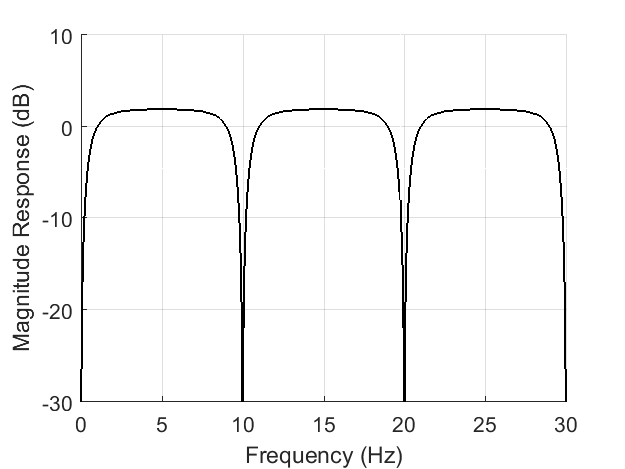
\includegraphics[width=\textwidth]{img/tau/mag_exp_5.png}
        \caption{Exponential~$\tau=5$}\label{fig:ExpTau5}
    \end{subfigure}
    \begin{subfigure}{.33\textwidth}
        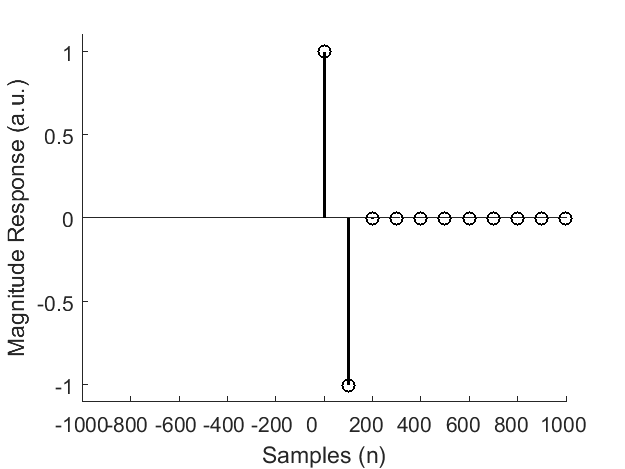
\includegraphics[width=\textwidth]{img/tau/kernel_exp_100.png}\\
        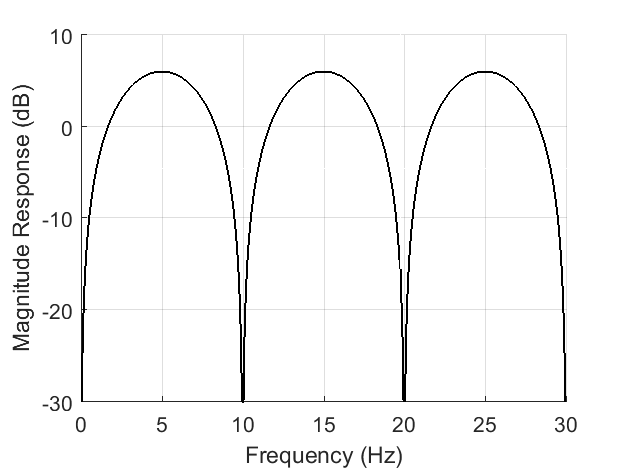
\includegraphics[width=\textwidth]{img/tau/mag_exp_100.png}
        \caption{Exponential~$\tau=100$}\label{fig:ExpTau100}
    \end{subfigure}
    \caption{Exemplary $\tau$ Tuning with $N=10$}\label{fig:ExemplaryTauTuning}
\end{figure}

In the limiting case of $\tau = 0$, the exponential kernel virtually converges with the uniform kernel~\figref{fig:ExpTau0}. Using a $\tau$ equal to the artifacts period length, the exponential kernel almost fully converges with the simple comb filter~\figref{fig:ExpTau100}. Note that very high $tau$ return an impulse response, and therefore just pass all signals.

\begin{figure}[hbtp]
    \begin{subfigure}{.33\textwidth}
        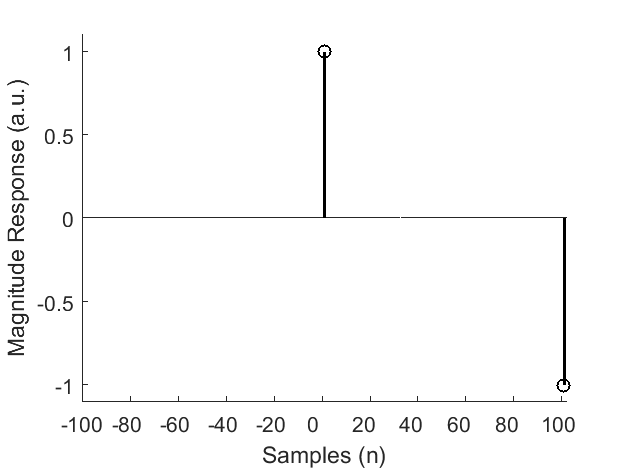
\includegraphics[width=\textwidth]{img/np/kernel_exp_1.png}\\
        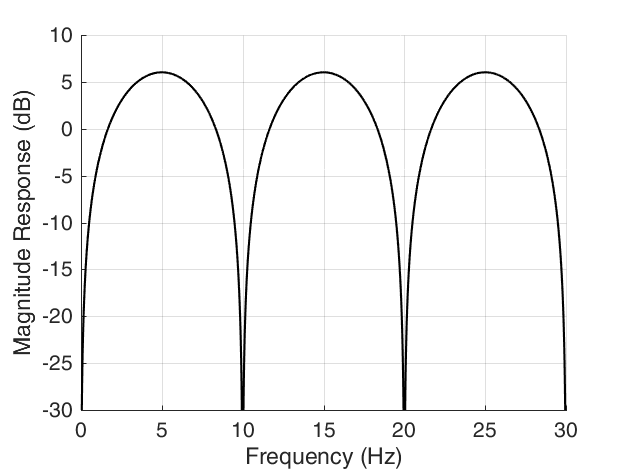
\includegraphics[width=\textwidth]{img/np/mag_exp_1.png}
        \caption{Exponential~$N=1$}\label{fig:ExNP1}
    \end{subfigure}
    \begin{subfigure}{.33\textwidth}
        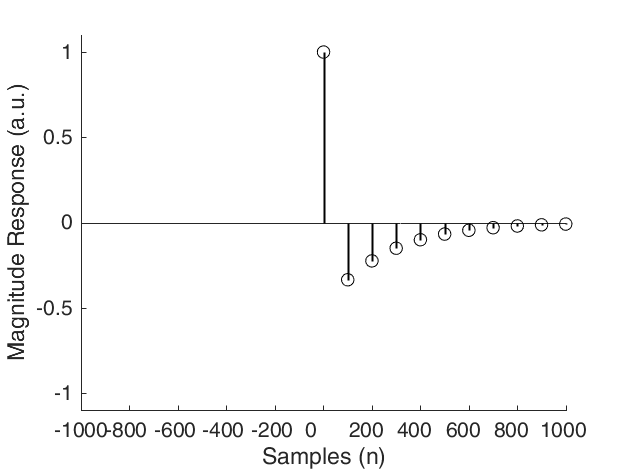
\includegraphics[width=\textwidth]{img/np/kernel_exp_10.png}\\
        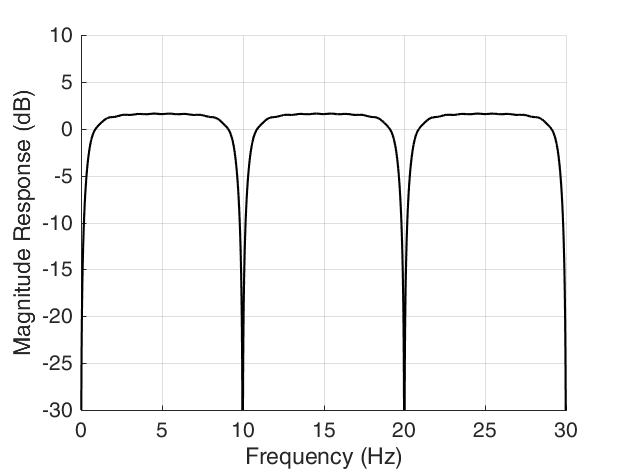
\includegraphics[width=\textwidth]{img/np/mag_exp_10.png}
        \caption{Exponential~$N=5$}\label{fig:ExpNP10}
    \end{subfigure}
    \begin{subfigure}{.33\textwidth}
        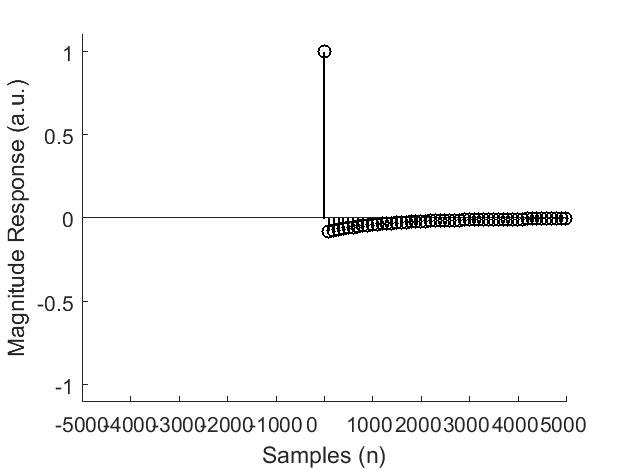
\includegraphics[width=\textwidth]{img/np/kernel_exp_50.png}\\
        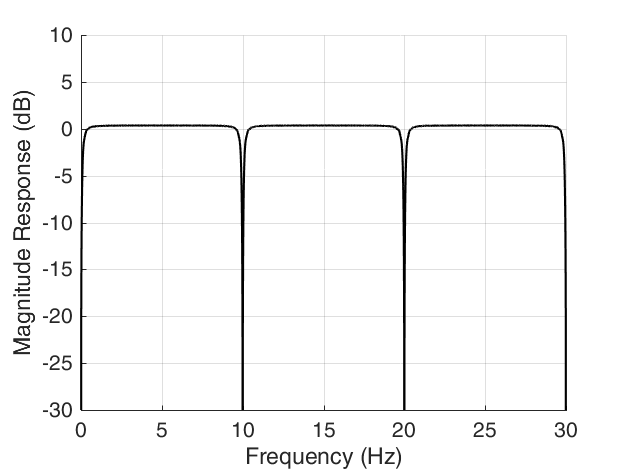
\includegraphics[width=\textwidth]{img/np/mag_exp_50.png}
        \caption{Exponential~$N=50$}\label{fig:ExpNP50}
    \end{subfigure}
    \caption{Exemplary $N$ Tuning with $\tau = 3$}\label{fig:ExemplaryNPTuning}
\end{figure}

In the limiting case of $N = 1$, we acquire the simple comb filter~\figref{fig:ExpTau1}. By increasing $N$ we achieve a flattening of the pass-band gain~\figref{fit:ExpNP50}.

\section{Evaluation}


First, we constructed a kernel based on the respective weighting functions~\eqref{eq:Weighted} and desired memory, or number of periods $N$. This kernel was then used to remove the artifact in a recording by convolution.
We wanted to evaluate the behavior of the filter in off-line analysis on simulated and real data and decided to use zero-padding for ease of computation.


\section{Conclusion}

One approach to model such a unknown dynamical system is with a Lévy-process. The key characteristics of such a process is that it is governed by randomness of the change between time-points. The increments are independent from each other, and are sampled from a continuous probability distribution with is stationary for the whole duration of the process. In that framework, the uncertainty of the estimate changes as a function of lag. Consider furthermore that we we only consider

Ornstein-Uhlenbeck-Prozess discrete time AR (1) process

\begin{equation}
    a(t+1) = a(t) + \theta(\mu-a(t)) + e(t+1)
\end{equation}
where $\left|\theta\right|<1$ and $\mu$ is the model mean.
Note that if the stochastic process is skewed or has a non-zero expectation value, the filter might need to add a constant for debiasing the estimation. If the stochastic process allows for jumps, small $N$ might return a more reliable estimation than large $N$.

Negative weights
This paper only dicusses real filter weights real, but complex weights might be a solution to tackle artifacts with periods that are not integer divisibles of the sampling frequency.

\bibliographystyle{apalike-oadoi}
\bibliography{sample}

\end{document}
